%-----------------------------------------------------------------------------
%
%               Template for sigplanconf LaTeX Class
%
% Name:         sigplanconf-template.tex
%
% Purpose:      A template for sigplanconf.cls, which is a LaTeX 2e class
%               file for SIGPLAN conference proceedings.
%
% Guide:        Refer to "Author's Guide to the ACM SIGPLAN Class,"
%               sigplanconf-guide.pdf
%
% Author:       Paul C. Anagnostopoulos
%               Windfall Software
%               978 371-2316
%               paul@windfall.com
%
% Created:      15 February 2005
%
%-----------------------------------------------------------------------------


\documentclass{sigplanconf}

% The following \documentclass options may be useful:

% preprint      Remove this option only once the paper is in final form.
% 10pt          To set in 10-point type instead of 9-point.
% 11pt          To set in 11-point type instead of 9-point.
% authoryear    To obtain author/year citation style instead of numeric.

\usepackage{amsmath}
\usepackage{amsfonts}
\usepackage{amssymb}
\usepackage{listings}
\usepackage{mathpartir}
\usepackage{graphicx}
\usepackage{comment}
\usepackage{pifont}
\usepackage{url}
\lstset
{
	basicstyle = \ttfamily\tiny,
	breaklines = true,
	frame = single
}


\begin{document}

\special{papersize=8.5in,11in}
\setlength{\pdfpageheight}{\paperheight}
\setlength{\pdfpagewidth}{\paperwidth}

\conferenceinfo{25th International Conference on Compiler Construction (CC 2016)}{March 17--18, 2016, Barcelona, Spain} 
\copyrightyear{2016} 
\copyrightdata{978-1-nnnn-nnnn-n/yy/mm} 
\doi{nnnnnnn.nnnnnnn}

% Uncomment one of the following two, if you are not going for the 
% traditional copyright transfer agreement.

%\exclusivelicense                % ACM gets exclusive license to publish, 
                                  % you retain copyright

%\permissiontopublish             % ACM gets nonexclusive license to publish
                                  % (paid open-access papers, 
                                  % short abstracts)

\titlebanner{banner above paper title}        % These are ignored unless
\preprintfooter{short description of paper}   % 'preprint' option specified.

\title{Building game scripting DSL's with the Metacasanova metacompiler}
\subtitle{}

\authorinfo{Francesco Di Giacomo \and Agostino Cortesi \and Mohamed Abbadi}
           {Universita' Ca' Foscari, Venezia}
           {francesco.digiacomo@unive.it \\ cortesi@unive.it \\
           	mohamed.abbadi@unive.it}
\authorinfo{Pieter Spronck}
           {Tilburg University}
           {p.spronck@uvt.nl}
\authorinfo{Giuseppe Maggiore}
		   {Hogeschool Rotterdam}
		   {maggg@hr.nl}

\maketitle

\begin{abstract}
Many video games rely on a Domain Specific Language (DSL) to implement
particular features such as artificial intelligence or time and
synchronization primitives.
Building a compiler for a DSL is a time-consuming task, and adding new
features to a DSL is hard  due to the low flexibility of the
implementation choice.
In this paper, we introduce an alternative to hand-made
implementations of compilers for DSLs  for game development: the
Metacasanova metacompiler.
We show the advantages of this metacomplier  in terms of simplicity of
designing and coding requirements, and in terms of  performance of the
resulting code, whose efficiency is comparable with hand-made
implementations in commercial general purpose languages.
\end{abstract}

\category{D.3.4}{Programming languages}{Processors}[Translator writing systems and compiler generators]

% general terms are not compulsory anymore, 
% you may leave them out
%\terms
%term1, term2

\keywords
metacompiler, compiler generator, Domain specific language, game development

\section{Introduction}
\label{sec:introduction}
The number of programming languages available on the market has dramatically increased during the last years. The tiobe index \cite{tiobe2018}, a ranking of programming languages based on their popularity, lists 50 programming languages for 2018. This number is only a small glimpse of the real amount, since it does not take into account several languages dedicated to specific applications. This growth has brought a further need for new compilers that are able to translate programs written in those languages into executable code. The goal of this work is to investigate how the development speed of a compiler can be boosted by employing meta-compilers, programs that generalize the task performed by a normal compiler. In particular the goal of this research is creating a meta-compiler that significantly reduces the amount of code needed to define a language and its compilation steps, while maintaining acceptable performance.

This chapter introduces the issue of expressing the solution of problems in terms of algorithms in Section \ref{sec:ch1_algorithms}. Then we proceed by defining how the semi-formal definition of an algorithm must be translated into code executable by a processor (Section \ref{sec:ch1_programming_languages}). In this section we discuss the advantages and disadvantages of using different kinds of programming languages with respect to their affinity with the specific hardware architecture and the scope of the domain they target. In Section \ref{sec:ch1_compilers} we explain the reason behind compilers and we explain why building a compiler is a time-consuming task. In Section \ref{sec:ch1_metacompilers} we introduce the idea of meta-compilers as a further step into generalizing the task of compilers. In this section we also explain the requirements, benefits, and the relevance as a scientific topic. Finally in Section \ref{sec:ch1_problem_statement} we formulate the problem statement and the research questions that this work will answer.

\section{Algorithms and problems}
\label{sec:ch1_algorithms}
Since the ancient age, there has always been the need of describing the sequence of activities needed to perform a specific task \cite{barbin2012history}, to which we refer with the name of \textit{Algorithm}. The allegedly most ancient known example of this dates back to the Ancient Greek, when Hero invented an algorithm to perform the factorization and the approximation of the square root, discovered also by other civilizations \cite{ bailey2012ancient, smith1923history} . Regardless of the specific details of each algorithm, one needs to use some kind of language  to define the sequence of steps to perform. In the past people used natural language to describe such steps but, with the advent of the computer era, the choice of the language has been strictly connected with the possibility of its implementation. Natural languages are not suitable for the implementation, as they are known to be verbose and ambiguous \cite{church1982coping, resnik1999semantic}. For this reason, several kind of formal solutions have been employed, which are described below.

\subsubsection*{Flow charts}
A flow chart is a diagram where the steps of an algorithm are defined by using boxes of different kinds, connected by arrows to define their ordering in the sequence. The boxes are rectangular-shaped if they define an \textit{activity} (or processing step), while they are diamond-shaped if they define a \textit{decision}. A rectangle with rounded corners denotes the initial step. An example of a flow chart describing how to sum the numbers in a sequence is described in Figure \ref{fig:ch1_flow_chart}.

\begin{figure}
	\centering
	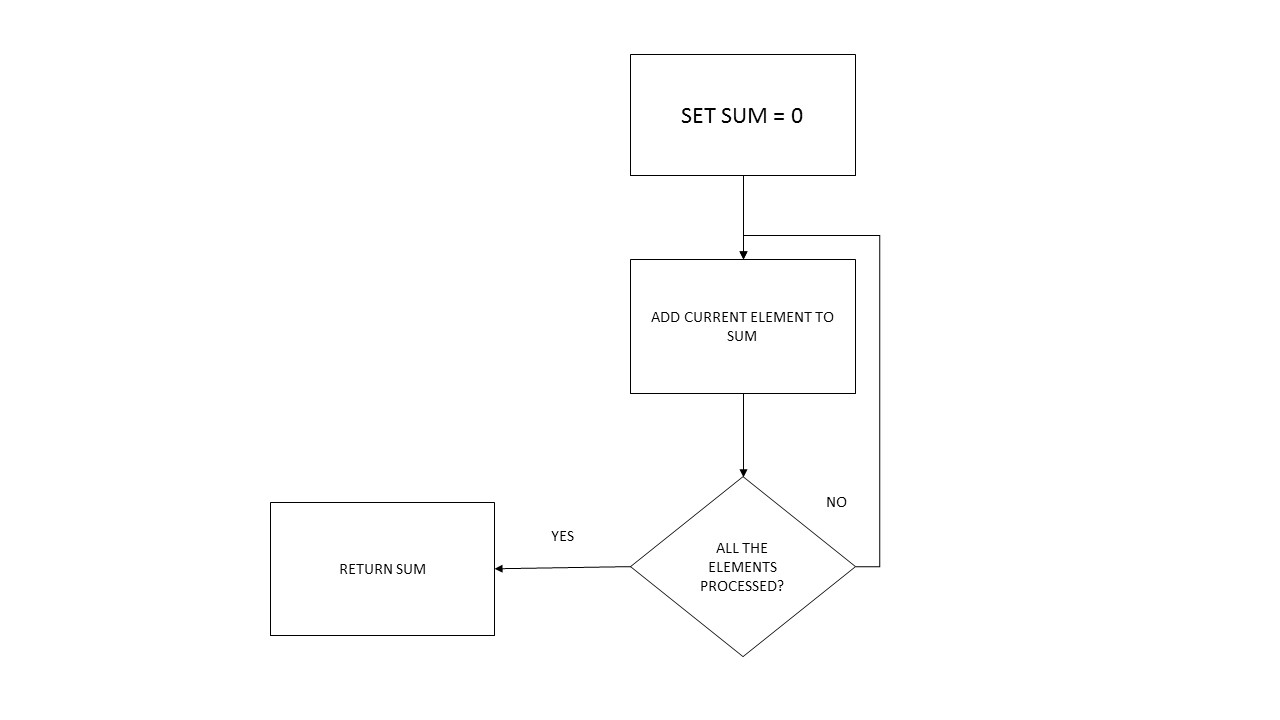
\includegraphics[width = \textwidth]{Figures/flow_chart}
	\caption{Flow chart for the sum of a sequence of numbers}
	\label{fig:ch1_flow_chart}
\end{figure}

\subsubsection*{Pseudocode}
Pseudocode is a semi-formal language that might contain also statements expressed in natural language and omits system specific code like opening file writers, printing messages on the standard output, or even some data structure declaration and initialization. It is intended mainly for human reading rather than machine reading. The pseudocode to sum a sequence of numbers is shown in Algorithm \ref{alg:ch1_pseudocode}.

\begin{algorithm}
	\caption{Pseudocode to perform the sum of a sequence of integer numbers}
	\label{alg:ch1_pseudocode}
	\begin{algorithmic}
		\Function{SumIntegers}{$l \text{ list of integers}$}
			\State $sum \gets 0$
			\ForAll {$x \text{ in } l$}
				\State $sum \gets sum + x$
			\EndFor
			\State \Return $sum$
		\EndFunction
	\end{algorithmic}
\end{algorithm}

\subsubsection*{Advantages and disadvantages}
Using flow charts or pseudo-code has the advantage of being able to define an algorithm in a way which is very close to the abstractions employed when using natural language: a flow chart combines both the use of natural language and a visual interface to describe an algorithm, pseudo-code allows to employ several abstractions and even define some steps in terms of natural language. The drawback of these two formal representations is that, when it comes to the implementation, the definition of the algorithm must be translated by hand into code that the hardware is able to execute. This could be done by implementing the algorithm in a low-level or high-level programming language. This process affects at different levels how the logic of the algorithm is presented, as explained further.

\section{Programming languages}
\label{sec:ch1_programming_languages}
A programming language is a formal language that is used to define instructions that a machine, usually a computer, must perform in order to produce a result through computation \cite{mordechai1996, narasimhan1967programming, oxford2008}. There is a wide taxonomy used to classify programming languages depending on their use \cite{kelleher2005lowering, myers1986visual, myers1990taxonomies}, but all can be grouped according to two main characteristics: the level of abstraction, or how close to the specific targeted hardware they are, and the domain, which defines the range of applicability of a programming language. In the following sections we give an exhaustive explanation of the aforementioned characteristics.

\subsection{Low-level programming languages}
\label{subsec:ch1_ll_languages}
A low-level programming language is a programming language that provides little to no abstraction from the hardware architecture of a processor. This means that it is strongly connected with the instruction set of the targeted machine, the set of instructions a processor is able to execute. These languages are divided into two sub-categories: \textit{first-generation} and \textit{second-generation} languages:

\subsubsection*{First-generation languages}
\textit{Machine code} falls into the category of first-generation languages. In this category we find all those languages that do not require code transformations to be executed by the processor. These languages were used mainly during the dawn of computer age and are rarely employed by programmers nowadays. Machine code is made of stream of binary data, that represents the instruction codes and their arguments \cite{guide2011intel, seal2001arm}. Usually this stream of data is treated by programmers in hexadecimal format, which is then remapped into binary code. The programs written in machine code were once loaded into the processor through a front panel, a controller that allowed the display and alteration of the registers and memory (see Figure \ref{fig:ch1_front_panel}). An example of machine code for a program that computes the sum of a sequence of integer numbers can be seen in Listing \ref{lst:ch1_machine_code}.

\begin{figure}
	\centering
	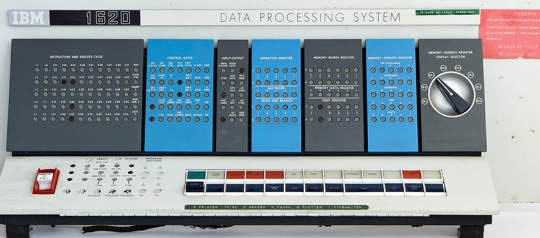
\includegraphics[width = \textwidth]{Figures/ch1_front_panel}
	\caption{Front panel of IBM 1620}
	\label{fig:ch1_front_panel}
\end{figure}

\begin{minipage}{\linewidth}
\begin{lstlisting}[numbers = left, caption = Machine code to compute the sum of a sequence of numbers, label = lst:ch1_machine_code]
 00075	c7 45 b8 00 00
 00 00
 0007c	eb 09	
 0007e	8b 45 b8
 00081	83 c0 01
 00084	89 45 b8
 00087	83 7d b8 0a
 0008b	7d 0f
 0008d	8b 45 b8
 00090	8b 4d c4
 00093	03 4c 85 d0
 00097	89 4d c4
 0009a	eb e2
\end{lstlisting}
\end{minipage}

\subsubsection*{Second-generation languages}
The languages in this category provides an abstraction layer over the machine code by expressing processor instructions with mnemonic names both for the instruction code and the arguments. For example, the arithmetic sum instruction \texttt{add} is the mnemonic name for the instruction code \texttt{0x00} in \texttt{x86} processors. Among these languages we find \textit{Assembly}, that is mapped with an \textit{Assembler} to machine code. The Assembler can load directly the code or link different \textit{object files} to generate a single executable by using a \textit{linker}. An example of assembly \texttt{x86} code corresponding to the machine code in Listing \ref{lst:ch1_machine_code} can be found in Listing \ref{lst:ch1_assembly_code}. You can see that the code in the machine code \texttt{00081	83 c0 01} at line 5 has been replaced by its mnemonic representation in Assembly as \texttt{add	eax, 1}.

\begin{minipage}{\linewidth}
\begin{lstlisting}[numbers = left, caption = Assembly x86 code to compute the sum of a sequence of numbers, label = lst:ch1_assembly_code]
mov	DWORD PTR _i$1[ebp], 0
jmp	SHORT $LN4@main
$LN2@main:
mov	eax, DWORD PTR _i$1[ebp]
add	eax, 1
mov	DWORD PTR _i$1[ebp], eax
$LN4@main:
cmp	DWORD PTR _i$1[ebp], 10			; 0000000aH
jge	SHORT $LN3@main
mov	eax, DWORD PTR _i$1[ebp]
mov	ecx, DWORD PTR _sum$[ebp]
add	ecx, DWORD PTR _numbers$[ebp+eax*4]
mov	DWORD PTR _sum$[ebp], ecx
jmp	SHORT $LN2@main
\end{lstlisting}
\end{minipage}

\subsubsection*{Advantages and disadvantages}
Writing a program in low-level programming languages might produce programs that are generally more efficient than their high-level counterparts, as ad-hoc optimizations are possible. However, the high-performance comes at great costs: (\textit{i}) the programmer must be an expert of the underlying architecture and of the specific instruction set of the processor, (\textit{ii}) the program loses portability because the low-level code is tightly bound to the specific hardware architecture it targets, (\textit{iii}) the logic and readability of the program is hidden among the details of the instruction set itself, and (\textit{iv}) developing a program in assembly requires a considerable effort in terms of time and debugging \cite{frampton2009demystifying}: assembly lacks any abstraction from the concrete hardware architecture, such as a type system, that partially ensures the correctness of the program or high-level constructs that allow to manipulate the execution of the program.

\subsection{High-level programming languages}
\label{subsec:ch1_hl_languages}
A high-level programming language is a programming language that offers a high level of abstraction from the specific hardware architecture of the machine. Unlike machine code (and in some way also assembly), high-level languages are not directly executable by the processor and they require some kind of translation process into machine code. The level of abstraction offered by the language defines how high level the language is. Several categories of high-level programming language exist, but the main one are described below.

\subsubsection*{Imperative programming languages}
\textit{Imperative programming languages} model the computation as a sequence of statements that alter the state of the program (usually the memory state). A program in such languages consists then of a sequence of \textit{commands}. Notable examples are FORTRAN, C, and PASCAL. An example of the program used in Listing \ref{lst:ch1_machine_code} and \ref{lst:ch1_assembly_code} written in C can be seen in Listing \ref{lst:ch1_c_code}. Line 5 to 9 corresponds to the Assembly code in Listing \ref{lst:ch1_assembly_code}.

\begin{lstlisting}[numbers = left, caption = C code to compute the sum of a sequence of numbers, label = lst:ch1_c_code]
int main()
{
  int numbers[10] = { 1, 6, 8, -2, 4, 3, 0, 1, 10, -5 };
  int sum = 0;
  for (int i = 0; i < 10; i++)
  {
    sum += numbers[i];
  }
  printf("%d\n", sum);
}
\end{lstlisting}

\subsection*{Declarative programming languages}
\textit{Declarative programming languages} are antithetical to those based on imperative programming, as they model computation as an evaluation of expressions and not as a sequence of commands to execute. Declarative programming languages are called as such when they are side-effects free or referentially transparent. The definition of referential transparency varies \cite{quine2013word}, but it is usually explained with the substitution principle, which states that a language is referentially transparent if any expression can be replaced by its value without altering the behaviour of the program \cite{mitchell2003concepts}. For instance, the following sentences in natural language are both true

\begin{lstlisting}
Cicero = Tullius

''Cicero`` contains six letters
\end{lstlisting} 

\noindent
but they are not referentially transparent, since replacing the last name with the middle name falsifies the second sentence.

A similar situation in programming languages is met when considering variable assignments: the statement

\begin{lstlisting}
x = x + 5
\end{lstlisting}

\noindent
is not referentially transparent. Let us assume this statement appears twice in a program and that at the beginning x = 0. Clearly the expression \texttt{x + 5} results in the value 5 the first time, but the second time the same statement is executed the expression has value 10. Thus replacing all the occurrences of \texttt{x + 5} with 5 is wrong, which is why imperative languages are not referentially transparent. A more rigorous definition of referential transparency can be found in \cite{sondergaard1990referential}.

Declarative programming languages are often compared to imperative programming languages by stating that declarative programming defines \textit{what} to compute and not \textit{how} to compute it. This family of languages include \textit{functional programming}, \textit{logic programming}, and \textit{database query languages}. Notable examples are F\#, Haskell, Prolog, SQL, and Linq (which is a query language embedded in C\#). Listing \ref{lst:ch1_fsharp_code_rec} shows the code to perform the sum of a sequence of integer numbers in F\# with a recursive function. Higher-order functions, such as \texttt{fold}, allow even to capture the same recursive pattern into a single function as shown in Listing \ref{lst:ch1_fsharp_code_fold}. Both implementations are referentially transparent.

\begin{lstlisting}[caption = Recursive F\# code to compute the sum of a sequence of numbers, label = lst:ch1_fsharp_code_rec]
let rec sumList l =
  match l with
  | [] -> 0
  | x :: xs -> x + (sumList xs)
\end{lstlisting}

\begin{lstlisting}[caption = F\# code to compute the sum of a sequence of numbers using higher-order functions, label = lst:ch1_fsharp_code_fold]
let sumList l = l |> List.fold (+) 0
\end{lstlisting}

\subsection{General-purpose vs Domain-specific languages}
\label{sec:ch1_dsl}
\textit{General-purpose languages} are defined as languages that can be used across different application domains and lack abstractions that specifically target elements of a single domain. Example of these are languages such as C, C++, C\#, and Java. Although several applications are still being developed by using general-purpose programming languages, in several contexts it is more convenient to rely on \textit{domain-specific languages}, because they offer abstractions relative to the problem domain that are unavailable in general-purpose languages \cite{van2000domain, voelter2013dsl}. Notable examples of the use of domain-specific languages are listed below.

\subsubsection*{Graphics programming}
Rendering a scene in a 3D space is often performed by relying on dedicated hardware. Modern graphics processors rely on shaders to create various effects that are rendered in the 3D scene. Shaders are written in domain-specific languages, such as GLSL or HLSL \cite{glhl2014, hlsl2018, hlslref2018}, that offer abstractions to compute operations at GPU level that are often used in computer graphics, such as vertices and pixel transformations, matrix multiplications, and interpolation of textures. Listing \ref{lst:ch1_hlsl_code} shows the code to implement light reflections in HLSL. At line 4 you can, for example, see the use of matrix multiplication provided as a language abstraction in HLSL.

\begin{lstlisting}[numbers = left, caption = HLSL code to compute the light reflection, label = lst:ch1_hlsl_code]
VertexShaderOutput VertexShaderSpecularFunction(VertexShaderInput input, float3 Normal : NORMAL)
{
  VertexShaderOutput output;
  float4 worldPosition = mul(input.Position, World);
  float4 viewPosition = mul(worldPosition, View);
  output.Position = mul(viewPosition, Projection);
  float3 normal = normalize(mul(Normal, World));
  output.Normal = normal;
  output.View = normalize(float4(EyePosition,1.0f) - worldPosition);
  return output;
}
\end{lstlisting}

\subsubsection*{Game programming}
Computer games are a field where domain-specific languages are widely employed, as they contain complex behaviours that often require special constructs to model timing event-based primitives, or to execute tasks in parallel. These behaviours cannot be modelled, for performance reasons, by using threads. Therefore, in the past, domain-specific languages which provide these abstractions have been implemented \cite{nwnlexicon2018, jass2011, unrealscript2018, sqf2018}. In Listing \ref{lst:ch1_sqf_code} an example of the SQF domain-specific language for the game ArmA2 is shown. This language offers abstractions to wait for a specific amount of time, to wait for a condition, and to spawn scripts that run in parallel to the callee, that you can respectively see at lines 18, 12, and 10.

\begin{lstlisting}[numbers = left, caption = ArmA 2 scripting language, label = lst:ch1_sqf_code]
"colorCorrections" ppEffectAdjust [1, pi, 0, [0.0, 0.0, 0.0, 0.0], [0.05, 0.18, 0.45, 0.5], [0.5, 0.5, 0.5, 0.0]];  
"colorCorrections" ppEffectCommit 0;  
"colorCorrections" ppEffectEnable true;

thanatos switchMove "AmovPpneMstpSrasWrflDnon";
[[],(position tower) nearestObject 6540,[["USMC_Soldier",west]],4,true,[]] execVM "patrolBuilding.sqf";
playMusic "Intro";

titleCut ["", "BLACK FADED", 999];
[] Spawn 
{
	waitUntil{!(isNil "BIS_fnc_init")};
	[
	  localize "STR_TITLE_LOCATION" ,
	  localize "STR_TITLE_PERSON",
	  str(date select 1) + "." + str(date select 2) + "." + str(date select 0)
	] spawn BIS_fnc_infoText;
	sleep 3;
	"dynamicBlur" ppEffectEnable true;   
	"dynamicBlur" ppEffectAdjust [6];   
	"dynamicBlur" ppEffectCommit 0;     
	"dynamicBlur" ppEffectAdjust [0.0];  
	"dynamicBlur" ppEffectCommit 7;
	titleCut ["", "BLACK IN", 5];
};
\end{lstlisting}

\subsubsection*{Shell scripting languages}
Shell scripting languages, such as the \textit{Unix Shell script}, are used to manipulate files or user input in different ways. They generally offer abstractions to the operating system interface in the form of dedicated commands. Listing \ref{lst:ch1_shell_code} shows an example of a program written in Unix shell script to convert an image from JPG to PNG format. At line 3 you can see the use of the statement \texttt{echo} to display a message in the standard output.

\begin{lstlisting}[numbers = left, caption = Unix shell code, label = lst:ch1_shell_code]
for jpg; do                                  
  png="${jpg%.jpg}.png"                    
  echo converting "$jpg" ...               
  if convert "$jpg" jpg.to.png ; then      
    mv jpg.to.png "$png"                 
  else                                     
    echo 'jpg2png: error: failed output saved in "jpg.to.png".' >&2
    exit 1
  fi                                       
done                                         
echo all conversions successful              
exit 0
\end{lstlisting}

\subsubsection*{Advantages and disadvantages}
High-level programming languages offer a variety of abstractions over the specific hardware the program targets. The obvious advantage of this is that the programmer does not need to be an expert of the underlying hardware architecture or instruction set. A further advantage is that the available abstractions are closer to the semi-formal description of the underlying algorithm as pseudo-code. This produces two desirable effects: (\textit{i}) the readability of the program is increased as the available abstractions are closer to the natural language than the equivalent machine code, and (\textit{ii}) that being able to mimic the semi-formal version of an algorithm, which is generally how the algorithm is presented and on which its correctness is proven, grants a higher degree of correctness in the specific implementation.

The use of a high-level programming language might, in general, not achieve the same high-performance as writing the same program with a low-level programming language  \cite{chatzigeorgiou2002evaluating}, but modern code-generation optimization techniques can generally mitigate this gap \cite{amarasinghe1993communication, wang2007code}. A further major issue in using high-level programming languages is that the machine cannot directly execute the code, thus the use of a compiler that translates the high-level program into machine code is necessary.

The portability of a high-level programming language depends on the architecture of the underlying compiler, thus some languages are portable and the same code can be run on different machines (for example Java), while others might require to be compiled to target a specific architecture (for example C++).

\section{Compilers}
\label{sec:ch1_compilers}
A compiler is a program that transforms source code defined in a programming language into another computer language, which usually is object code but can also be code in a high-level programming language \cite{aho2007compilers, appel2002javacompiler}. Writing a compiler is a necessary step to implementing a high-level programming language. Indeed, a high-level programming language, unlike low-level ones, are not executable directly by the processor and need to be translated into machine code, as stated in Section \ref{subsec:ch1_ll_languages} and \ref{subsec:ch1_hl_languages}.

The first complete compiler was developed by IBM for the FORTRAN language and required 18 person-years for its development \cite{backus1957fortran}. This clearly shows that writing a compiler is a hard and time-consuming task.

A compiler is a complex piece of software made of several components that implement a step in the translation process. The translation process performed by a compiler involves the following steps:

\begin{enumerate}
	\item \textit{syntactical analysis:} In this phase the compiler checks that the program is written according to the grammar rules of the language. In this phase the compiler must be able to recognize the \textit{syntagms} of the language (the ``words'') and also check if the program conforms to the syntax rules of the language through a grammar specification.
	\item \textit{type checking:} In this phase the compiler checks that a \textit{syntactically correct program} performs operations conform to a defined \textit{type system}. A type system is a set of rules that assign properties called types to the constructs of a computer program \cite{pierce2002types}. The use of a type system drastically reduces the chance of having bugs in a computer program \cite{cardelli1996type} . This phase can be performed at compile time (\textit{static typing}) or the generated code could contain the code to perform the type checking at runtime (\textit{dynamic typing}). 
	\item \textit{code generation:} In this phase the compiler takes the \textit{syntactically and type-correct program} and performs the translation step. At this point an equivalent program in a target language will be generated. The target language can be object code, another high-level programming language, or even a bytecode that can be interpreted by a virtual machine.
\end{enumerate}

All the previous steps are always the same regardless of the language the compiler translates from and they are not part of the creative aspect of the language design \cite{book1970cwic}. Approaches to automating the construction of the syntactical analyser are well known in literature \cite{mcpeak2004elkhound, nivre2006maltparser, parr1995antlr}, to the point that several lexer/parser generators are available for programmers, for example all those belonging to the \texttt{yacc} family such as \texttt{yacc} for C/C++, \texttt{fsyacc} for F\#, \texttt{cup} for Java, and \texttt{Happy} for Haskell. On the other hand, developers lack a set of tools to automate the implementation of the last two steps, namely the type checking and the code generation.

For this reason, when implementing a compiler, the formal type system definition and the operational semantics, which is tightly connected to the code generation and defines how the constructs of the language behave, must be translated into the abstractions provided by the host language in which the compiler will be implemented. Other than being a time-consuming activity itself, this causes that (\textit{i}) the logic of the type system and operational semantics is lost inside the abstraction of the host-language, and (\textit{ii}) it is difficult to extend the language with new features.

\section{Meta-compilers}
\label{sec:ch1_metacompilers}
In Section \ref{sec:ch1_compilers} we described how the steps involved in designing and implementing a compiler do not require creativity and are always the same, regardless of the language the compiler is built for. The first step, namely the syntactical analysis, can be automated by using one of the several lexer/parser generators available, but the implementation of a type checker and a code generator still relies on a manual implementation. This is where meta-compilers come into play: a meta-compiler is a program that takes the source code of another program written in a specific language and the language definition itself, and generates executable code. The language definition is written in a programming language, referred to as \textit{meta-language}, which should provide the abstractions necessary to define the syntax, type system, and operational semantics of the language, in order to implement all the steps above.

\subsection{Requirements}
As stated in Section \ref{sec:ch1_metacompilers}, a meta-compiler should provide a meta-language that is able to define the syntax, type system, and operational semantics of a programming language. In Section \ref{sec:ch1_compilers} we discussed how methods to automate the implementation of syntactical analyser are already known in scientific literature. For this reason, in this work, we will focus exclusively on automating the implementation of the type system and of the operational semantics. Given this focus, we formulate the following requirements:

\begin{itemize}
	\item The meta-language should provide abstractions to define the constructs of the language. This includes the possibility of defining control structures, operators with any form of prefix or infix notation, and the priority of the constructs that is used when evaluating their behaviour. Furthermore, it must be possible to define the equivalence of language constructs. For instance, an integer constant might be considered both a value and a basic arithmetic expression.
	
	\item The meta-language must be able to mimic as close as possible the formal definition of a programming language. This will bring the following benefits: (\textit{i}) Implementing the language in the meta-compiler will just involve re-writing almost one-to-one the type system or the semantics of the language with little or no change; (\textit{ii}) the correctness and soundness \cite{cardelli1996type, milner1972proving} of the language formal definition will be directly reflected in the implementation of the language; indeed if a meta-program allows to mimic directly the type system and semantics of the language their correctness is transferred also in the implementation, while this might not be trivial when translating them in the abstractions of a high-level programming language; (\textit{iii}) any extension of the language definition can be just added as an additional rule in the type system or the semantics.
	
	\item The meta-compiler must be able to embed libraries from external languages, so that they can be used to implement specific behaviours such as networking transmission or specific data structure usage.
\end{itemize}

\subsection{Benefits}
\label{sec:ch1_benefits}
%list the benefits first and then explain. Add a paragraph also about correctness
Programming languages usually are released with a minimal (but sufficient to be Turing-complete) set of features, and later extended in functionality in successive versions. This process tends to be slow and often significant improvements or additions are only seen years after the first release. For example, Java was released in 1996 and lacked an important feature such as Generics until 2004, when J2SE 5.0 was released. Furthermore, Java and C++ lacked constructs from functional programming, which is becoming more and more popular with the years \cite{thompson1995miranda}, such as lambda abstractions until 2016, while a similar language like C\# 3.0 was released with such capability in 2008. The slow rate of change of programming languages is due to the fact that every abstraction added to the language must be reflected in all the modules of its compiler: the grammar must be extended to support new syntactical rules, the type checking of the new constructs must be added, and the appropriate code generation must be implemented. Given the complexity of compilers, this process requires a huge amount of work, and it is often obstructed by the low flexiblity of the compiler as piece of software. Using a meta-compiler would speed up the extension of an existing language because it would require only to change on paper the type system and the operational semantics, and then add the new definitions to their counterpart written in the meta-language. This process is easier because the meta-language should mimic as close as possible their behaviour. Moreover, backward compatibility is automatically granted because an older program will simply use the extended language version to be compiled by the meta-compiler.

To this we add the fact that, in general, for the same reasons, the development of a new programming language is generally faster when using a meta-compiler. This could be beneficial to the development of a high variety of domain-specific languages. Indeed, such languages are often employed in situations where the developers have little or no resources to develop a fully-fledged hard-coded compiler by hand. For instance, it is desirable for game developers to focus on aspects that are strictly tied to the game itself, for example the development of an efficient graphics engine or to improve the game logic. At the same time they would need a domain-specific language to express some behaviours typical of games, things that could be achieved by using a meta-compiler rather than on a hand-made implementation.

\subsection{Scientific relevance} %change the tile
\label{sec:ch1_scientific_relevance}
Meta-compilers have been researched since the 1960's \cite{schorre1964meta} and several implementations have been proposed \cite{ braborovansky1998overview, venboer2008stratego, klint2009rascal, pettersson1996compiler, verdejo2006executable}. In general meta-compilers perform poorly compared to hard-coded compilers because they add the additional layer of abstraction of the meta-language. Moreover, a specific implementation of a compiler opens up the possibility of implementing language-specific optimizations during the code generation phase. Meta-compilers have been used in a wide range of applications, such as source code analysis and manipulation and physical simulations \cite{kaagedal1998generating}, but no use up to our knowledge was made in the field of domain-specific languages for games. Since games are pieces of software that are very demanding in terms of performance, we think that it could be of interest to investigate the applicability of meta-compilers in the scope of domain-specific languages for games and the development speed up introduced by the use of such a tool. In this work we present Metacasanova, a meta-compiler based on natural semantics that was born from the intent of easing the development of the domain-specific language for game development Casanova, and we analyse the benefit of using it for a re-implementation and extension of Casanova.

\section{Problem statement}
\label{sec:ch1_problem_statement}
In Section \ref{sec:ch1_programming_languages} we showed the advantages of using high-level programming languages when implementing an algorithm. Among such languages, it is sometimes desirable to employ domain-specific languages that offer abstractions relative to a specific application domain (Section \ref{sec:ch1_dsl}). In Section \ref{sec:ch1_compilers} we described the need of a compiler for such languages, and that developing one is a time-consuming activity despite the process being, in great part, non-creative. In Section \ref{sec:ch1_metacompilers} we introduced the role of meta-compilers to speed up the process of developing a compiler and we listed the requirements and the benefits that one should have. In Section \ref{sec:ch1_scientific_relevance} we explained why we believe that meta-compilers are a relevant scientific topic if coupled with the problem of of developing domain-specific languages in response to the their increasing need. We can now formulate our problem statement:

\vspace{0.5cm}
\noindent
\textbf{Problem statement: } \textit{\psContent}

\vspace{0.5cm}
\noindent
The first parameter we need to evaluate in order to answer this question is the size of the code reduction needed to implement the domain-specific language. At this purpose, the following research question arises:

\vspace{0.5cm}
\noindent
\textbf{Research question 1: } \textit{\rqContentOne}

\vspace{0.5cm}
\noindent
The second parameter we need to evaluate is the eventual performance loss caused by introducing the abstraction layer provided by the meta-compiler. This leads to the following research question:

\vspace{0.5cm}
\noindent
\textbf{Research question 2: } \textit{\rqContentTwo}

\vspace{0.5cm}
\noindent
In case of a performance loss, we need to identify the cause of this performance loss and if an improvement is possible. This leads to the following research question:

\vspace{0.5cm}
\noindent
\textbf{Research question 3: } \textit{\rqContentThree}

\vspace{0.5cm}
\noindent

\section{Thesis structure}
This thesis describes the architecture of Metacasanova, a meta-compiler whose meta-language is based on operational semantics, and a possible optimization for such meta-compiler. It also shows its the capabilities by implementing a small imperative language and re-implementing the existing domain-specific language for games \textit{Casanova 2}, extending it with abstractions to express network operations for multiplayer games.

In Chapter \ref{ch:background} we provide background information in order to understand the choices made for this work. The chapter presents the state of the art in designing and implementing compilers and existing research on meta-compilers.

In Chapter \ref{ch:metacasanova} we present the architecture of Metacasanova by extensively describing the implementation of all its modules.

In Chapter \ref{ch:languages} we show how to use Metacasanova to implement two languages: a small imperative language, and \textit{Casanova 2}, a language for game development. At the end of the chapter we provide an evaluation of the performance of the two languages and their implementation length with respect to existing compilers, thus answering to Research Question 1 and 2.

In Chapter \ref{ch:functors} we discuss the performance loss of the implementation of the presented languages and we propose an extension of Metacasanova that aims to improve the performance of the generated code, thus answering Research Question 3.

In Chapter \ref{ch:functor_languages} we show how to use functors to improve the performance of Casanova implemented in Metacasanova, comparing this approach and the one presented in Chapter \ref{ch:languages} with respect to the execution time of a sample in Casanova. 

In Chapter \ref{ch:networking} we propose an extension of Casanova 2 for multiplayer game development. We first provide its hard-coded compiler solution and then we show how to extend the implementation in the meta-compiler to include the same extension. In this chapter we evaluate the performance of a multiplayer game implemented in Casanova with this extension with respect to the same game implemented in C\#, and we measure the effort of realising such extension in the hard-coded compiler of Casanova versus the implementation with Metacasanova.

In Chapter \ref{ch:discussion} we discuss the result and answer the research questions.


\section{The challenges of building a game DSL}
\label{sec:problem_statement}
In this section we introduce the general architecture of a game. We then present an example of common timing and synchronization primitives used in DSL's for games and we show some techniques typically used to implement them. For each technique we list the main drawbacks. Finally we present our solution to the problem of developing a DSL for games.

\subsection{Preliminaries}
A game engine is usually made by several interoperating components. All the components use a shared data structure, called \textit{game state}, for their execution. The two main components of a game are the \textit{logic engine}, which defines how the game state evolves during the game execution, and the \textit{graphics enginge}, which draws the scene by reading the updated game state. These two components are executed in lockstep within a function called \textit{game loop}. The game loop is executed indefinitely, updating the game state by calling the logic engine, and drawing the scene by using the graphics engine. An iteration of the game loop is called \textit{frame}. Usually a game should run between 30 to 60 frames per second. This requires both the graphics engine and the logic engine to be high-performance. In this paper we will only take into account the performance of the logic engine, as scripting drives the logic of the game loop. A schematic representation of this architecture can be seen in Figure \ref{fig:game_loop}.

\begin{figure}
	\centering
	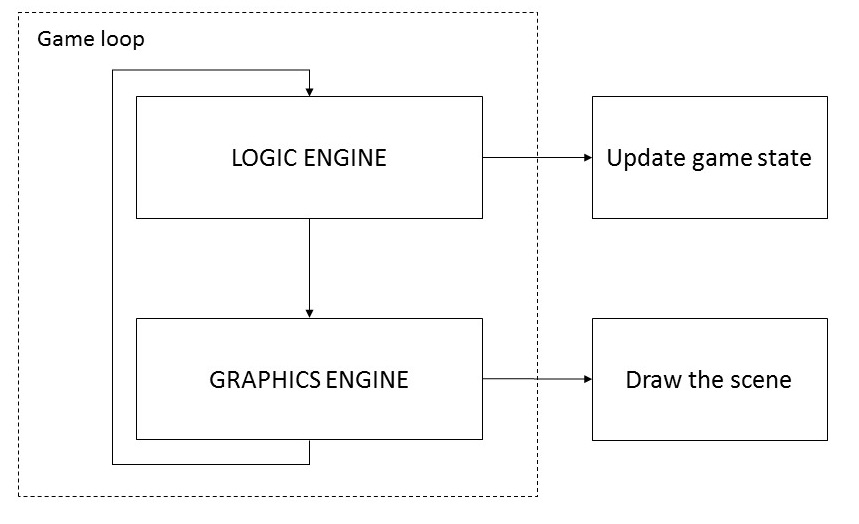
\includegraphics[scale=0.3]{Pictures/game_loop}
	\caption{Game loop}
	\label{fig:game_loop}
\end{figure}

\subsection{A time and synchronization primitive}
\label{subsec:synchronization}
A common requirement in game DSL's is a statement which allows to pause the execution of a function for a specified amount of time or until a condition is met. We will refer to these statements as \texttt{wait} and \texttt{when}. Such a behaviour can be modelled using different techniques:

\begin{itemize}
	\item \textit{Threads} allow to solve such synchronization problems but they are unsuitable for video game development because of memory usage and CPU overhead due to their scheduling.
	\item \textit{Finite State Machines} allow to represent such concurrent behaviours \cite{CASANOVA2_PAPER} by using a \texttt{switch} control structure to an opportune state. For instance in the case of timed wait, the states are \textit{wating} and \texttt{clear} (when the timer has elapsed). This solution is high-performance but the logic of the behaviour is lost inside the \texttt{switch} structure.
	\item \textit{Strategy pattern} allows to represent the instructions of the language has polymorphic data types. Each concurrent structure is implemented by a class which defines the behaviour of the current structure, and the next structure to execute. This solution is not high-performance due to virtuality and the high number of object instantiations.
	\item \textit{Monadic DSL} uses a variation of the state monad. It represents scripts with two states: \textit{Done} and \textit{Next}. The bind operator is used to simulate the code interruption. This approach is simple and elegant but it suffers of the same virtuality problems of the strategy pattern, this time because of the extensive use of lambda expressions.
	\item \textit{Compiled DSL} is the most common solution and allows to represent the concurrency by using concurrent control structures defined in the language. Compiled DSL's grant high-performance and code readability, but they require to implement a compiler or an interpreter for it.
\end{itemize}

In what follows we show a possible implementation of these statements using the presented techniques. We deliberately ignore the thread-based implementation since, as explained above, threads are not suitable for game development.

\paragraph{Monadic DSL:} A possible approach to building an interpreted DSL is using monads in a functional programming language, as done in \cite{CASANOVA1_PAPER}. A script is a function that takes no input parameters and returns the state of the script after the execution of the current statement. The state can be either \textit{Done}, when the script terminates, or \textit{Next} when the script is still running and we need to pass the rest of the script to be evaluated. We present a definition of the monad in the following code snippet in pseudo-ml:

\begin{lstlisting}
type Script<'a> = Unit -> State<'a>
and State<'a> = Done of 'a | Next of Script<'a>
\end{lstlisting}

\noindent
We can define the \texttt{Return} and \texttt{Bind} operators as follow:

\begin{lstlisting}
let return (x : 'a) : Script<'a> =
  fun () -> Done x
  
let (p : Script<'a>) >>= (k : 'a -> Script<'b>) : Script<'b> =
  fun () ->
    match p with
    | Done x -> k x ()
    | Next p' -> Next(p' >>= k)
\end{lstlisting}

\noindent
The \texttt{Return} operator simply returns a script that builds the result of the computation. The \texttt{Bind} operator checks the current state of the script: if the script has terminated then it simply builds the result by executing the last script statement, otherwise it returns the continuation containing the invocation of the \texttt{Bind} on the remaining part of the script. In this framework the \texttt{wait} statement can be implemented as follows (we assume that \texttt{do} is a shortcut for the bind on a function returning \texttt{Script<Unit>}):

\begin{lstlisting}
let yield : Script<Unit> =
  fun () -> Next(fun () -> Done ())

let rec waitRecursion (interval : float32, 
                       startingTime : float32) : Script<Unit> =
  let t = getTime()
  let dt = (t - t0)
  if dt < interval then
    do yield
    do waitRecursion(startingTime)
  else
    return ()
      
let wait (timer : float32) : Script<Unit> =
  let t0 = getTime()
  do waitRecursion(timer, t0)
  
let when (predicate : Unit -> bool) : Script<Unit> =
  if predicate () then return ()
  else
    do yield
    do when predicate
\end{lstlisting}
\noindent
The \texttt{yield} function simply forces the script to stop for one frame. The \texttt{wait} function recursively checks if the timer has elapsed. If this is not the case it skips a frame and then re-evaluates otherwise it returns \texttt{Unit}. \texttt{wait} on a predicate simply skips a frame and keeps re-executing itself until the condition is met.

\paragraph{Strategy pattern} Implementing \texttt{wait} and \texttt{when} with the strategy pattern requires to define an interface which contains the signature for a method to run the script. Usually scripts need to access the time elapsed between the current frame and the previous one and to a reference to the game state data structure for various reasons, which are passed as parameter for this method. The method returns the updated script after the current execution. We present the code for the interface in a pseudo-C\# code:

\begin{lstlisting}
public interface Script
  public Script Run(float dt, GameState state);
\end{lstlisting}

We will then model \texttt{wait} and \texttt{when} with two classes implementing such interface. Each of the script commands contains a reference to the next statement to execute.

\begin{lstlisting}
public class Wait : Statement
  private Statement next;
  private float time;
  
  public Script Run(float dt, GameState state)
    if (time >= 0)
      time -= dt;
      return this;
    else
      return next;

public class When : Statement
  private Func<bool> predicate;
  private Script next;
  
  public Script Run(float dt, GameState state)
    if (predicate())
      return next;
    else
      return this;
\end{lstlisting}

\paragraph{Finite state machines:} In this approach we model \texttt{wait} and \texttt{when} as finite state automata. Both statements require to store the state of the automata. \texttt{wait} requires to store a timer whose value is updated at each frame. \texttt{when} stores a predicate to execute and check at every game logic update. \texttt{wait} has three states: (\textit{i}) timer initialization, (\textit{ii}) check timer and update, and (\textit{iii}) timer elapsed. In the first state we initialize the timer and then update it for the first time. The second state is used to check whether the timer has elapsed. The third state is used to continue with the execution after the time has elapsed.

\begin{lstlisting}
//WAIT
public void Update(float dt, GameState gameState)
  switch(state)
    case -1: 
      this.t = timer;
      state = 0;
      goto case 0;
    case 0:
      this.t = this.t - dt
      if (this.t <= 0)
        state = 1;
        goto case 1:
      else
        return;
    case 1:
    //run the code after wait
\end{lstlisting}

\texttt{when} has two states: (\textit{i}) check predicate, (\textit{ii}) predicate satisfied (go on with the execution). The first state checks if the predicate has been satisfied. If that is the case, we jump to the next state, otherwise we pause the execution and we remain in the same state.

\begin{lstlisting}
//WHEN
public void Update(float dt, GameState gameState)
  switch(state)
    case 0:
      if (predicate())
        state = 1;
        goto case 1:
      else
        return;
    case 1:
    //run the code after when
\end{lstlisting}

\paragraph{Waiting with a hard-coded compiler:} This approach requires to build a compiler by generating the syntax using a standard lexer/parser generator. After that usually it is required to define a set of type rules, and the operational semantics of the language constructs. The type rules and the operational semantics are then implemented in the type checker and the code generator of the compiler.

\subsection{Discussion}
In the previous paragraph we have seen different techniques employed by developers to implement timing and synchronization statements commonly used in video games. We now list the advantages and disadvantages of each solution:

\begin{itemize}
	\item \textit{Monadic DSL:} this solution is elegant but inefficient, because of the extensive use of lambda expressions in monads. Indeed lambdas are usually implemented with virtual method calls. The code to define a monadic DSL is compact.
	\item \textit{Strategy Pattern:} this solution is simple but low-performance because of the virtual method calls the logic update must invoke to run the statements and the high number of object instantiation to generate the script statements (one per statement). Besides the readability of the program for long scripts is lost due to the long chain of object instantiations. A library supporting scripts implemented with the strategy pattern is compact.
	\item \textit{Finite state machines:} this approach is high-performance due to the small overhead of the \texttt{switch} control structure. Unfortunately the logic of the program for very complex scripts with several nested synchronizations is lost inside huge \texttt{switch} structures and the complexity increases drastically with the number of interruptions and synchronizations in the script \cite{AI_GAMES}. Moreover note that for each timer we have to maintain a separate timer, and for any of the two control structures we need to store the state of the automaton. Implementing complex synchronizations require long and complex state machines.
	\item \textit{Hard-coded compiler:} this approach is high-performance, as we could generate the state machines presented above during the code generation step, but building, maintaining, and extending a hard-coded compiler is a hard and time-consuming task. The code length increases with the size of the compiler (in term of modules and code lines) and the language complexity.
\end{itemize}
This situation is summarized in Table \ref{tab:techniques}.

\begin{table}
	\small
	\centering
	\begin{tabular}{|c|c|c|c|}
		\hline
		Technique & Readability & Performance & Code length \\
		\hline
		Monadic DSL & \checkmark & \ding{55} & \checkmark \\
		\hline
		Strategy Pattern & \ding{55} & \ding{55} & \checkmark \\
		\hline
		Finite state machines & \ding{55} & \checkmark & \ding{55} \\
		\hline
		Hard-coded compiler & \checkmark & \checkmark & \ding{55} \\
		\hline
	\end{tabular}
	\caption{Pros and cons of script implementation techniques}
	\label{tab:techniques}
\end{table}

In this work we propose another development approach in building a game DSL by using a metacompiler, a program which takes as input a language definition, a program written in that language, and generates executable code.

\noindent
Given this considerations, we formulate the following problem statement.

\vspace{0.5cm}
\noindent
\textbf{PROBLEM STATEMENT:}
Given the formal definition of a game DSL our goal is to automate, by using a metacompiler, the process of building a compiler for that language in a (\textit{i}) short (code lines), (\textit{ii}) clear (code readability), and (\textit{iii}) efficient (time execution) way, with respect to a hand-made implementation.



\section{The Metacasanova metacompiler}
\label{sec:formal_description}
In this section we show how \texttt{wait} and \texttt{when} can be expressed with type and semantics rules. We show how this rules are implemented in a hard-coded compiler. We then introduce the idea of the metacompiler, explaining the advantage over a hard-coded compiler. We give an informal overview of the Metacasanova metacompiler and we then proceed to formalize its syntax and semantics.

\subsection{Type and semantics of wait and when}
Usually the type and semantics rules of language elements are represented by rules that resemble those of logic models. Each rule is made of a set of \textit{premises} and a \textit{conclusion}.

\begin{mathpar}
	\inferrule
	{premise_{1} \\\\ premise_{2} \\\\ ... \\\\ premise_{n}}
	{conclusion}
\end{mathpar}

The conclusion is true if all the premises are true. According to this model, the type rules for \texttt{wait} and \texttt{when} are the following ($E \vdash x \; : \; T$ means that $x$ has type $T$ in the environment $E$):

\begin{mathpar}
	\inferrule
	{E \vdash t \; : \; \mathtt{float}}
	{E \vdash \mathtt{wait} \; t \; : \; \mathtt{void}}
	
	\inferrule
	{E \vdash c \; : \; \mathtt{bool}}
	{E \vdash \mathtt{when} \; c : \; \mathtt{void}}
\end{mathpar}

\noindent
while their operational semantics is (with $\langle expr \rangle$ we mean ``evaluating $exp$'', with ; a sequence of statements, and with $dt$ the time difference between the current frame and the previous):

\begin{mathpar}
	\inferrule
	{\langle t - dt > 0 \rangle \; \Rightarrow \; \texttt{true}}
	{\langle \mathtt{wait} \; t;k \; dt \rangle \; \Rightarrow \; \langle \mathtt{wait} \; t - dt ; k \; dt \rangle}
	
	\inferrule
	{\langle t - dt > 0 \rangle \; \Rightarrow \; \texttt{false}}
	{\langle \mathtt{wait} \; t ; k \; dt \rangle \; \Rightarrow \; \langle k \; dt \rangle}
\end{mathpar}

\begin{mathpar}
	\inferrule
	{\langle c \rangle \; \Rightarrow \; \mathtt{true}}
	{\langle \mathtt{when} \; c;k \; dt \rangle \; \Rightarrow \; \langle k \; dt\rangle}
	
	\inferrule
	{\langle c \rangle \; \Rightarrow \; \mathtt{false}}
	{\langle \mathtt{when} \; c;k \; dt \rangle \; \Rightarrow \; \langle \mathtt{when} \; c;k \; dt \rangle}
\end{mathpar}

\subsection{Implementation in a hard-coded compiler}
The semantics rules of \texttt{wait} and \texttt{when} can be implemented into the type checker module of a compiler written in a general purpose language. We assume that these two statements are represented as a discriminated union in the language AST as shown by the following pseudo-ml code snippet:

\begin{lstlisting}
type Statement =
| Wait of Expression
| When of Expression
...
\end{lstlisting}

The rules are evaluated by means of a recursive function. In the case of a \texttt{wait} statement, we first type check its argument. If the argument is a float than we return the node in the type-checked AST corresponding to the type-checked \texttt{wait}. If the argument has another type then we raise an exception since the argument has not a valid type. In the case of a \texttt{when} statement we do the same, but this time we check that the argument has boolean type.

\begin{lstlisting}
let rec typecheckStatement ( stmt : Statement ) : TypedStatement =
match stmt with
  | Wait ( expr ) ->
    let exprType = typecheckExpr expr
    match exprType with
	| Float -> Wait ( FloatExpr )
	| _ -> failwith (" Expected Float but given " + exprType . ToString ())
  | When ( expr ) ->
	let exprType = typecheckExpr expr
	match exprType with
	| Boolean -> Wait ( BoolExpr )
	| _ -> failwith (" Expected Boolean but given " + exprType . ToString ())
...
\end{lstlisting}

The code generation part requires to output code according to the semantics rules defined above. In this step the compiler can, for example, generate state machines implementing the behaviour described in Section \ref{subsec:synchronization}.

\subsection{Motivation for Metacasanova}

From the example above we can see that, regardless of the implemented language, the process of type checking and implementing the operational semantics in a hard-coded compiler, is repetitive. Indeed, building the type checker and the code generator of a hard-coded compiler is a single, fixed translation of these rules into the general purpose language that was chosen for the implementation. This process can be summarized by the following behaviour:

\begin{itemize}
	\item Find a rule which conclusion matches the structure of the language we are analysing.
	\item Recursively evaluate all the premises in the same way.
	\item When we reach a rule with no premises (a base case), we generate a result (which might be the type of the structure we are evaluating or code that implements its operational semantics).
\end{itemize}

Our goal is to take this process and automate it, starting only from the specifications which the hard-coded compiler would implement.

In the following sections we define the requirements the \textit{Metacasanova} metacompiler must satisfy. We present informally the structure of a program in Metacasanova. We then proceed in defining the formal syntax in BNF of Metacasanova grammar. Finally we define the semantics of Metacasanova.

\subsection{Requirements of Metacasanova}
In order to relieve programmers of manually defining the behaviour described above in the back-end of the compiler, we propose to use a metacompiler. This metacompiler must include the following features:

\begin{itemize}
	\item It must be possible to define custom operators (or functions) and data containers. This is needed to define the syntactic structures of the language we are defining.
	\item It must be typed: each syntactic structure can be associated to a specific type in order to be able to detect meaningless terms (such as adding a string to an integer) and notify the error.
	\item It must be possible to have polymorphic syntactical structures. This is useful to define equivalent ``roles'' in the language for the same syntactical structure; for instance we can say that an integer literal is both a \textit{Value} and an \textit{Arithmetic expression}.
	\item It must natively support the evaluation of semantics rules, as those shown above. A \textit{rule},in Metacasanova, in the fashion of a logic rule, is made of a sequence of premises and a conclusion. The premises can be function calls or clauses. Clauses are boolean expressions that are checked in order to proceed with the rule evaluation. The function call will run in order all the rules that contain that function as conclusion. The return value of the first rule that succeeds is taken. A rule returns a value if all the clauses evaluate to \texttt{true} and all the function calls succeed.
\end{itemize}

From this specifications, we see that our goal is indeed a metacompiler, as it takes as input a language definition, a program for that language, and outputs runnable code that mimics the code that a hard-coded compiler would output.

\subsection{General overview}

A Metacasanova program is made of a set of \texttt{Data} and \texttt{Function} definitions, and a sequence of rules. A data definition specifies the constructor name of the data type (used to construct the data type), its field types, and the type name of the data. Optionally it is possible to specify a priority for the constructor of the data type. For instance this is the definition of the sum of two arithmetic expression

\begin{lstlisting}
Data Expr -> "+" -> Expr : Expr  Priority 500
\end{lstlisting}

\noindent
Note that Metacasanova allows you to specify any kind of notation for data types in the language syntax, depending on the order of definition of the argument types and the constructor name. In the previous example we used an infix notation. The equivalent prefix and postfix notations would be:

\begin{lstlisting}
Data "+" -> Expr -> Expr : Expr
Data Expr -> Expr -> "+" : Expr
\end{lstlisting}

\noindent
A function definition is similar to a data definition but it also has a return type. For instance the following is the evaluation function definition for the arithmetic expression above:

\begin{lstlisting}
Func "eval" -> Expr : Evaluator => Value
\end{lstlisting}

\noindent
In Metacasanova it is also possible to define polymorphic data in the following way:

\begin{lstlisting}
Value is Expr
\end{lstlisting}

\noindent
In this way we are saying that an atomic value is also an expression and we can pass both a composite expression and an atomic value to the evaluation function defined above.

Metacasanova also allows to embed C\# code into the language by using double angular brackets. This code can be used to embed .NET types when defining data or functions, or to run C\# code in the rules. For example in the following snippets we define a floating point data which encapsulates a floating point number of .NET to be used for arithmetic computations:

\begin{lstlisting}
Data "$f" -> <<float>> : Value
\end{lstlisting}

\noindent
A rule in Metacasanova, as explained above, may contain a sequence of function calls and clauses. In the following snippet we have the rule to evaluate the sum of two floating point numbers:

\begin{lstlisting}
eval a => $f c
eval b => $f d
<<c + d>> => res
------------------------
eval (a + b) => $f res
\end{lstlisting}

\noindent
Note that if one of the two expressions does not return a floating point value, then the entire rule evaluation fails. Also note that we can embed C\# code to perform the actual arithmetic operation. Metacasanova selects a rule by means of pattern matching in order of declaration on the function arguments. This means that both of the following rules will be valid candidates to evaluate the sum of two expressions:

\begin{lstlisting}
...
---------------
eval expr => res

...
----------------
eval (a + b) => res
\end{lstlisting} 

In Metacasanova it is also possible to branch rule evaluation if more than one rule is suitable to evaluate the function call. In this case we will generate a list of results based on all the possible execution branches. In order to achieve this we use the operator \texttt{==>} instead of \texttt{=>}.

Finally the language supports expression bindings with the following syntax:

\begin{lstlisting}
x := $f 5
\end{lstlisting}

\subsection{Syntax in BNF}
The following is the syntax of Metacasanova in Backus-Naur form. Note that, for brevity, we omit the definitions of typical syntactical elements of programming languages, such as literals or identifiers:

\begin{lstlisting}
<program> ::= 
  {<include>} {<import>} {<data>} <function> {<function>} {<alias>} <rule> {<rule>}
<premise> ::= 
  <clause> | <functionCall> | <binding>
<binding> ::= 
  id ":=" <constructor>
<rule> ::= 
  {premise} "-" {"-"} <functionCall>
<clause> ::= //typical boolean expression
<functionCall> ::= 
  <id> {<argument>} <arrow> <argument> | 
  {<argument>} <id> {<argument>} <arrow> <argument> | 
  <id> {<argument>} <arrow> <argument>
<arrow> ::= "=>" | "==>"
<constructor> ::= 
  <id> {<argument>} | 
  {<argument>} <id> {<argument>} | 
  {<argument>} <id>
<external> ::= "<<" <csharpexpr> ">>"
<csharpexpr> ::= //all available C# expressions
<argument> ::= 
  ["("] 
    (<id> | 
    <external> | 
    <literal> | 
    <constructor>) 
  [")"]
<literal> ::= //typical literals such as integer, float, string, ...
<import> ::= import id {"." id}
<include> ::= include id {.id}
<alias> ::= <typeDef> is <typeDef>
<typeDef> ::= id | "<<" id ">>"
<typeArguments> :: = 
  '"' <id> '"' {"->" <typeDef>} ":" <typeDef> |
  <typeDef> {"->" <typeDef>} "->" '"' <id> '"' {"->" <typeDef>} ":" <typeDef> |
  <typeDef> {"->" typeDef} "->" '"' <id> '"' ":" <typeDef> 
<function> ::= Func <typeArguments> "=>" <typeDef> [Priority <literal>]
<data> ::= Data <typeArguments> [Priority <literal>]
\end{lstlisting}

\subsection{Semi-formal Semantics}
In what follows we assume that the pattern matching of the function arguments in a rule succeeds, otherwise a rule will fail to return a result.
The informal semantics of the rule evaluation in Metacasanova is the following:
\begin{enumerate}
	\item[R1] A rule with no clauses or function calls always returns a result.
	\item[R2] A rule returns a result if all the clauses evaluate to \texttt{true} and all the function calls in the premise return a result.
	\item[R3] A rule fails if at least one clause evaluates to \texttt{false} or one of the function calls fails (returning no results).
\end{enumerate}
We will express the semantics, as usual, in the form of logical rules, where the conclusion is obtained when all the premises are true.
In what follows we consider a set of rules defined in the Metacasanova language $R$. Each rule has a set of function calls $F$ and a set of clauses (boolean expressions) $C$. We use the notation $f^{r}$ to express the application of the function $f$ through the rule $r$. We will define the semantics by using the notation $\langle expr \rangle$ to mark the evaluation of an expression, for example $\langle f^{r} \rangle$ means evaluating the application of $f$ through $r$. Note that the result of evaluating $f$ through $r$ produces generally a set of results because of the branching operator described above. In the base case R1 we return a single result because a rule without premises cannot branch. The following is the formal semantics of the rule evaluation in Metacasanova, based on the informal rules defined above:


\begin{mathpar}
	\mprset{flushleft}
	\inferrule*[left=R1:]
	{C = \emptyset \\\\ F = \emptyset}
	{\langle f^{r} \rangle \Rightarrow x} \\

	\mprset{flushleft}
	\inferrule*[left=R2:]
	{\forall c_{i} \in C \;, \langle c_{i} \rangle \Rightarrow true \\\\
	 \forall f_{j} \in F \; \exists r_{k} \in R \; | \; \langle f_{j}^{r_{k}} \rangle \Rightarrow \lbrace x_{k_{1}}, x_{k_{2}}, ..., x_{k_{m}} \rbrace}
	{\langle f^{r} \rangle \Rightarrow \lbrace x_{1}, x_{2}, ..., x_{n} \rbrace} \\
	
	\mprset{flushleft}
	\inferrule*[left=R3(a):]
	{\exists c_{i} \in C \; | \; \langle c_{i} \rangle \Rightarrow false}
    {\langle f^{r} \rangle \Rightarrow \emptyset} \\
    
    \mprset{flushleft}
    \inferrule*[left=R3(b)]
    {\forall r_{k} \in R \; \exists f_{j} \in F \; | \; \langle f_{j}^{r_{k}} \rangle \Rightarrow \emptyset}
    {\langle f^{r} \rangle \Rightarrow \emptyset}
\end{mathpar}

R1 says that, when both $C$ and $F$ are empty (we do not have any clauses or function calls), the rule in Metacasanova returns a result. R2 says that, if all the clauses in $C$ evaluates to true and, for all the function calls in $F$ we can find a rule that returns a result (all the function applications return a result for at least one rule of the program), then the current rules return a result. R3(a) and R3(b) specify when a rule fails to return a result: this happens when at least one of the clauses in $C$ evaluates to false, or when one of the function applications does not return a result for any of the rules defined in the program.


\section{Case study: Casanova 2.5, a language for game development}
\label{sec:casanova3}
In this section we will briefly introduce the Casanova language, a domain specific language for games. We then show a re-implementation, which we call Casanova 2.5, of the Casanova 2 language hard-coded compiler as an example of use of Metacasanova.

\subsection{The Casanova language}
Casanova 2.5 is a language oriented to video game development which is based on Casanova 2 \cite{CASANOVA2_PAPER}. A program in Casanova is a tree of \textit{entities}, where the root is marked in a special way and called \textit{world}. Each entity is similar to a \textit{class} in an object-oriented programming language: it has a constructor and some fields. The fields do not have access modifiers because they are not directly modifiable from the code except with a specific statement. Each entity also contains a list of \textit{rules}, that are methods that are ticked in order with a specific refresh rate called \texttt{dt}. Each rule takes as input four elements: \texttt{dt}, \texttt{this}, which is a reference to the current entity, \texttt{world} that is a reference to the world entity, and a subset of entity fields called \textit{domain}. A rule can only modify the fields contained in the domain. The rules can be paused for a certain amount of seconds or until a condition is met by using the \texttt{wait} statement. It is possible to modify the values of the fields in the domain by using the \texttt{yield} statement which takes as input a tuple of values to assign to the fields. When the \texttt{yield} statement is executed the rule is paused until the next frame. Also the body of control structures (\texttt{if-then-else}, \texttt{while}, \texttt{for}) is interruptible. In the following section we show the implementation of Casanova 2.5 in Metacasanova.

\subsection{Casanova 2.5}
The memory in Casanova 2.5 is represented using three maps, where the key is the variable/field name, and the value is the value stored in the variable/field. The first dictionary represents the global memory (the fields of the \texttt{world} entity or \textit{Game State}), the second dictionary represents the current entity fields, and the third the variable bindings local to each rule.

The core of the entity update is the \texttt{tick} function. This function evaluates in order each rule in the entity by calling the \texttt{evalRule} function. This function executes the body of the rule and returns a result depending on the set of statements that has been evaluated. This result is used by \texttt{tick} to update the memory and rebuild the rule body to be evaluated at the next frame. The result of \texttt{tick} is a \texttt{State} containing the rules updated so far, and the updated entity and global fields. Since a rule must be restarted after the whole body has been evaluated, we need to store a list containing the original rules, which will be restored when evaluation returns \texttt{Done} (see below). At each step the function recursively calls itself by passing the remaining part of original rules (the rules which body was not altered by the evaluation of the statements) and modified rules (which body has been altered by the evaluation of the statements) to be evaluated. The function stops when all the rules have been evaluated, and this happens when both the original and the modified rule lists are empty.

Interruption is achieved by using \textit{Continuation passing style}: the execution of a sequence of statements is seen as a sequence of steps that returns the result of the execution and the remaining code to be executed. Every time a statement is executed we rebuild a new rule whose body contains the continuation which will be evaluated next. 

\begin{comment}
For example, consider the following rule:

\begin{lstlisting}
rule X,Y =
  while X > 0 do
    wait 1.0f
    yield X - 1,Y + 1
\end{lstlisting}

The code is executed atomically until the \texttt{wait} statement (assuming that the \texttt{while} condition is true). At that point we rebuild a new rule containing the code to execute at the next iteration:

\begin{lstlisting}
rule X,Y =
  wait (1.0f - dt)
  yield X - 1, Y + 1
  while X > 0 do
    wait 1.0f
    yield X - 1,Y + 1
\end{lstlisting}
Note that the \texttt{while} is placed at the end of the continuation because it must be re-evaluated after the first iteration is complete, and that we have decreased the waiting time by \texttt{dt} (the time elapsed between one frame and the previous one).
\end{comment}

The possible results returned by the \texttt{tick} function are the following: (\textit{i}) \texttt{Suspend} contains a \texttt{wait} statement with the updated timer, the continuation, and a data structure called \texttt{Context} which contains the updated local variables, the entity fields, and the global fields. The function rebuilds a rule which body is the sequence of statements contained by the \texttt{Suspend} data structure. (\textit{ii})\texttt{Resume} is returned when the timer must resume after the last waited frame. In order not to skip a frame we must still re-evaluate the rule at the next frame and not immediately. In this case the argument of \texttt{Resume} is only the remaining statements to be executed. (\textit{iii}) \texttt{Yield} stops evaluation for one frame. We use the continuation to rebuild the rule body. Memory is updated by \texttt{evalRule}. (\textit{iv})\texttt{Done} stops the evaluation for one frame and rebuilds the original rule body by taking it from the original rules list.

For brevity we write only the code for \texttt{Suspend}. A full implementation can be found at \cite{CASANOVA_SOURCE_CODE}. You can see a schematic representation of the tick function in Figure \ref{fig:tick}.

\begin{lstlisting}
evalRule (rule dom body k locals delta) fields globals => Suspend (s;cont) (Context newLocals newFields newGlobals)
r := rule dom s cont newLocals dt
tick originals rs newFields newGlobals dt => State updatedRules updatedFields updatedGlobals
st := State (r::updatedRules) updatedFields updatedGlobals
------------------------------------------------------
tick (original::originals) ((rule dom body k locals delta)::rs) fields globals dt => st
\end{lstlisting}


\begin{figure}
	\centering
	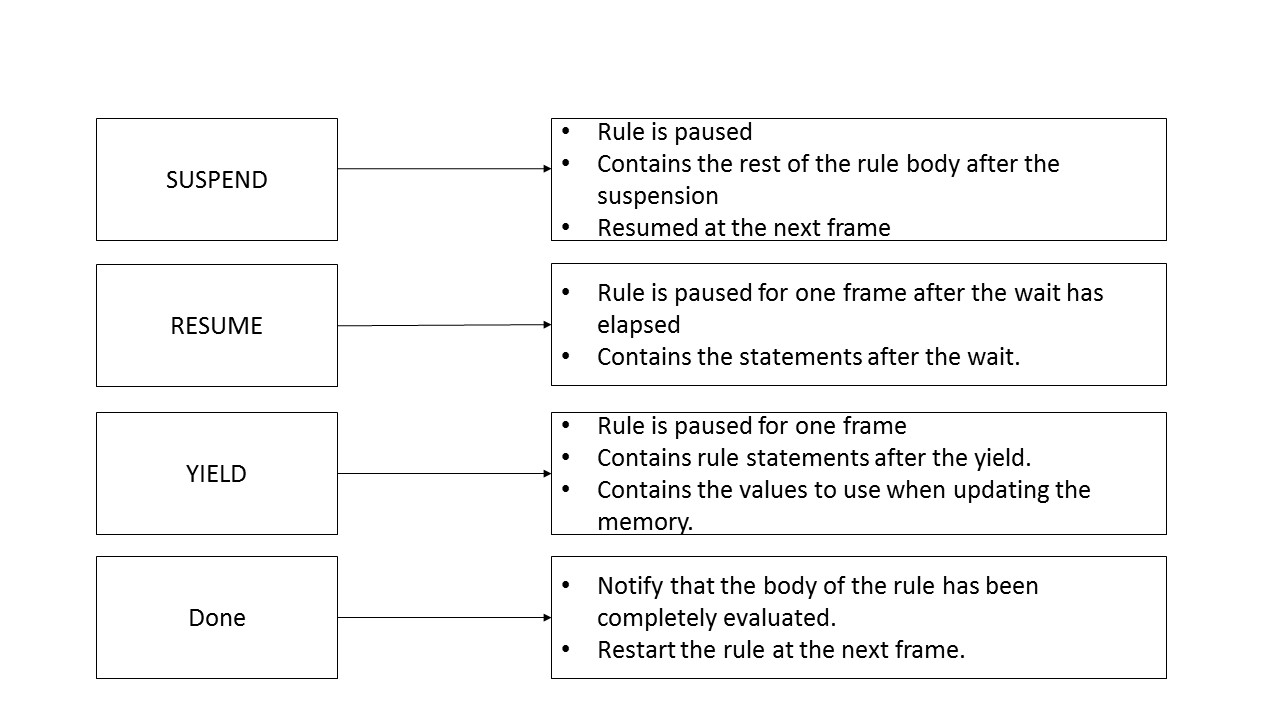
\includegraphics[scale = 0.4]{Pictures/tick2}
	\caption{Casanova 2.5 rule evaluation}
	\label{fig:tick}
\end{figure}

The function \texttt{evalRule} calls \texttt{evalStatement} to evaluate the first statement in the body of the rule passed as argument. The result of the evaluation of the statement is processed in the following way: (\textit{i}) if the result is \texttt{Done}, \texttt{Suspend} or \texttt{Resume} then it is just returned to the caller function. We omit the code for this case, since it is trivial; (\textit{ii}) if the result is \texttt{Atomic} it means that the evaluated statement was uninterruptible and the remaining statements of the rule must be re-evaluated immediately; (\textit{iii}) if the result is \texttt{Yield} then the fields in the domain are updated recursively in order and then the updated memory is encapsulated in the \texttt{Yield} data structure and passed to the caller function.

\begin{lstlisting}
evalStatement b k ctxt dt => Atomic z c    
evalRule (rule dom z nop c dt) => res
-------------------------------
evalRule (rule dom b k ctxt dt)  => res
\end{lstlisting}

\begin{lstlisting}
evalStatement b k (Context locals fields globals) dt => Yield ks values context
updateFields dom values context  => updatedContext
--------------------------------------------------------
evalRule (rule dom b k locals dt) fields globals => Yield ks values updatedContex
\end{lstlisting}

Note that, in case of a rule containing only atomic statements, we will eventually return \texttt{Done} after having recursively called \texttt{evalStatement} for all the statements, and the rule will be paused for one frame.

\begin{comment}
\begin{figure}
	\centering
	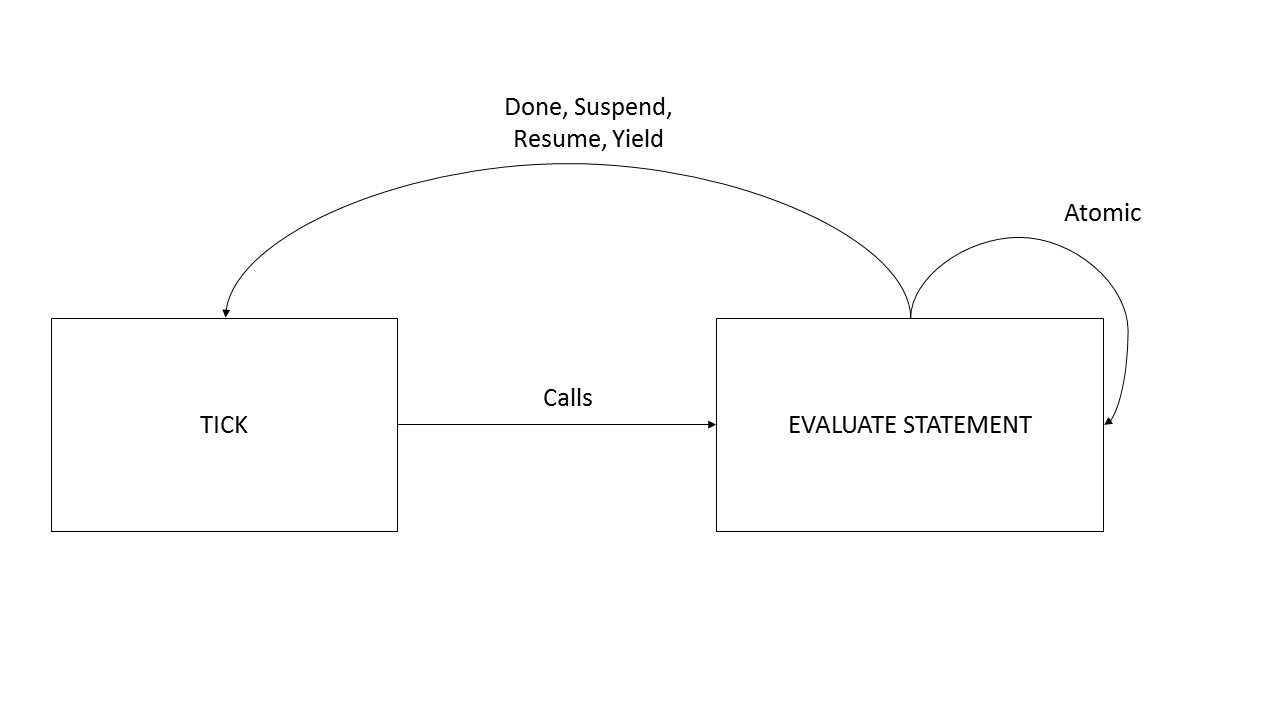
\includegraphics[scale=0.15]{Pictures/statement_evaluation}
	\caption{Statement evaluation}
	\label{fig:statement_evaluation}
\end{figure}
\end{comment}

\noindent
The \texttt{evalStatement} function is used both to evaluate a single statement and a sequence of statements. When evaluating a sequence of statements, the first one is extracted. A continuation is built with the following statement and passed to a recursive call to \texttt{evalStatement} which evaluates the extracted statement. If the existing continuation is non-empty, then it is added before the current continuation. If both the continuation and the body are empty (situation represented by the \texttt{nop} operator) then it means the rule evaluation has been completed and we return \texttt{Done}.

\begin{lstlisting}
a != nop
---------------------                           ----------------------- 
addStmt a b => a;b                              addStmt nop nop => nop   

addStmt b k => cont
evalStatement a cont ctxt dt => res
-------------------------------                 -----------------------------------       
evalStatement (a;b) k ctxt dt => res            evalStatement nop nop ctxt dt => Done ctxt


\end{lstlisting}

\noindent
We will now present, for brevity, only the evaluation of the \texttt{wait} and \texttt{yield} statements. Both the evaluation of the control structures and the variable bindings always return \texttt{Atomic} because they do not, by definition, pause the execution of the rule.

The \texttt{wait} statement has two different evaluations, based on the rules defined in Section \ref{sec:problem_statement}: (\textit{i}) the timer has elapsed: in this case we return \texttt{Resume} which contains the code to execute after the \texttt{wait} statement, or (\textit{ii}) the timer has not elapsed: in this case we return \texttt{Suspend} which contains the \texttt{wait} statement with the updated timer followed by the continuation.


\begin{lstlisting}
<<t <= dt>> == false
----------------------------------
evalStatement (wait t) k ctxt dt => Suspend wait <<t - dt>>;k ctxt

<<t <= dt>> == true
----------------------------------
evalStatement (wait t) k ctxt dt => Resume k ctxt
\end{lstlisting}

\noindent
The \texttt{yield} statement takes as argument a list of expressions whose values are used to update the corresponding fields in the rule domain. The evaluation rule recursively evaluates the expressions and stores them into a list passed as argument of the \texttt{Yield} result. Those arguments are used later by \texttt{evalRule} to update the corresponding fields.

\begin{lstlisting}
eval expr ctxt => v
evalYield exprs ctxt => vs
-------------------------------------------          ----------------------------
evalYield (expr :: exprs) ctxt => v :: vs            evalYield nil ctxt => nil
\end{lstlisting}


\section{Evaluation}
\label{sec:evaluation}
GrandeOmega has been tested extensively with students from Hogeschool Rotterdam, a university of applied science in the Netherlands. The classes were divided into two groups: in the first classes were given some programming assignments to be completed in the traditional way (without GrandeOmega), while in the second other classes were asked to solve the assignments both in the traditional way and in GrandeOmega. Table \ref{tab:performance_go} and Figure \ref{fig:bar_chart} contain data relative to the pass rate and average grades of the classes that were asked to used also GrandeOmega, with and without using it. Table \ref{tab:prediction} and Figure \ref{fig:prediction} contain data relative to the accuracy of the prediction on the student success performed by GrandeOmega. The total number of students who participated is 241.

The data shows that the use of GrandeOmega enhanced the pass rate of classes 1B and 1C, but not that of 1F, 1L, and 1A. This means that the students of 1B and 1C failed questions in the traditional way that they were able to solve in GrandeOmega. Nonetheless, we can see that it always enhanced the grades of all the classes by at least 4\%. Moreover, if we compare the average passing grade of these classes with those who never used GrandeOmega, we can see that we reach a difference of even 12\%.

GrandeOmega was revealed to be effective even in predicting the success of students with a total reliability of 77\%, based on the percentage of assignment completed correctly.

\begin{table}[!h]
	\begin{tabular}{|p{0.1\columnwidth}|p{0.1\columnwidth}|p{0.1\columnwidth}|p{0.1\columnwidth}|p{0.1\columnwidth}|p{0.1\columnwidth}|}
		\hline
		\textbf{Class} & Completions & Pass rate & Pass rate G.O. & Average grade & Average grade G.O. \\
		\hline
		INF1B & 71.8 & 3 & 14 & 84.7 & 97.2 \\
		\hline
		INF1F & 56.7 & 6 & 5 & 77.0 & 88.1 \\
		\hline
		INF1L & 48.1 & 2 & 2 & 75 & 83.8 \\
		\hline
		INF1A & 41.7 & 7 & 7 & 82.1 & 86.5 \\
		\hline
		INF1C & 35.6 & 5 & 7 & 82.5 & 93.3 \\
		\hline
	\end{tabular}
	\caption{Student performance before and after GrandeOmega}
	\label{tab:performance_go}
\end{table}

\begin{table}[!h]
	\begin{tabular}{|p{0.2\textwidth}|p{0.2\textwidth}|p{0.2\textwidth}|p{0.2\textwidth}|p{0.2\textwidth}|}
		\hline
		\textbf{Class} & \textbf{Correct prediction} & \textbf{False positive} & \textbf{False negative} & \textbf{Incorrect prediction} \\
		\hline
		INF1B & 16 & 8 & 2 & 10 \\
		\hline
		INF1F & 11 & 2 & 4 & 6 \\
		\hline
		INF1L & 18 & 3 & 1 & 4 \\
		\hline
		INF1A & 13 & 0 & 2 & 2 \\
		\hline
		INF1C & 15 & 1 & 1 & 2 \\
		\hline
	\end{tabular}
	\caption{Prediction of student performance}
	\label{tab:prediction}
\end{table}

\begin{table}[!h]
	\begin{tabular}{|p{0.25\textwidth}|p{0.25\textwidth}|p{0.25\textwidth}|p{0.25\textwidth}|}
		\hline
		\textbf{Class} & \textbf{Average grade} & \textbf{Passed students} & \textbf{Avarage passing grade} \\
		\hline
		INF1H & 41.4 & 3 & 83.3 \\
		\hline
		INF1E & 30.6 & 1 & 75 \\
		\hline
		INF1J & 23.3 & 0 & N.A. \\
		\hline
		INF1G & 41.4 & 7 & 80.3 \\
		\hline
	\end{tabular}
	\caption{Results of classes without GrandeOmega}
	\label{tab:performance_no_go}
\end{table}

\begin{figure}[!h]
	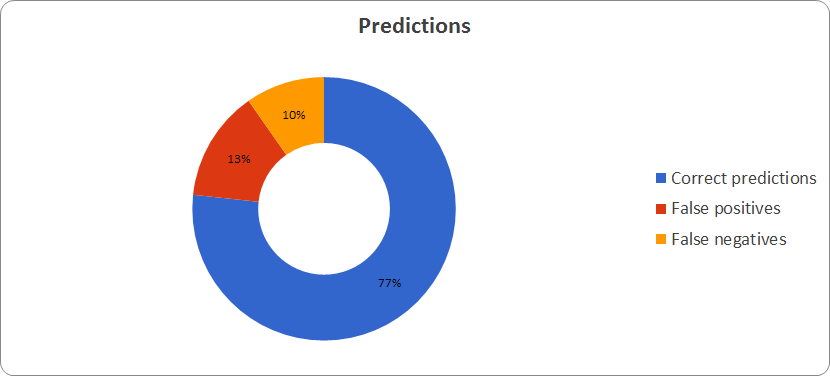
\includegraphics[width = \columnwidth]{Figures/prediction}
	\caption{Predition accuracy of GrandeOmega}
	\label{fig:prediction}
\end{figure}

\begin{figure}[!h]
	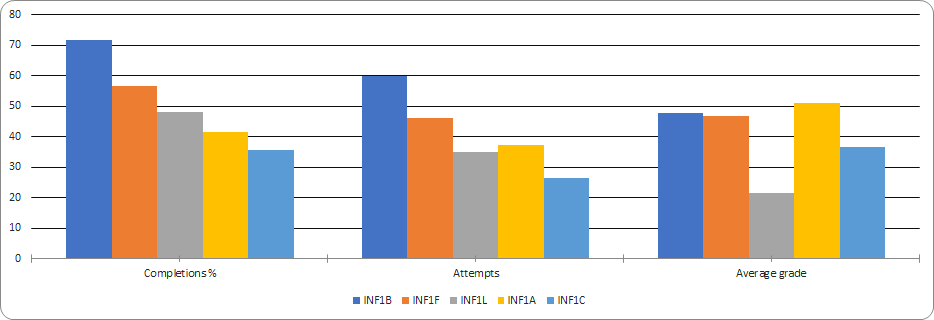
\includegraphics[width = \columnwidth]{Figures/bar_chart}
	\caption{Student performance with and without G.O.}
	\label{fig:bar_chart}
\end{figure}


\section{Conclusion and future work}
\label{sec:future_works}
In this work we addressed the problem of teaching and learning how to program and we proposed the use of a didactic model called GrandeOmega. The web implementation of GrandeOmega was tested on a subset of students from Hogeschool Rotterdam with promising results: the use of the didactic model managed, in some cases, to improve the pass rate of the students, while it always improved their overall performance (measured as a percentage of the maximum score). Furthermore, the classes that did not use GrandeOmega performed generally more poorly to the point that, in one of them, no students managed to successfully complete any of the assignments. The tool is also able to predict with a reliability of 77\% if a student will pass the course on the base of the amount of completed assignments. We can thus conclude that using GrandeOmega boosts the general performance of the students, measured as the percentage of correctly given answers, and, in some cases, improves also the pass rate of the course. On the other hand, students who did not use GrandeOmega at all performed, on average, worse and had a lower passing percentage.

\bibliography{bibliography}
\bibliographystyle{abbrvnat}



\end{document}

%                       Revision History
%                       -------- -------
%  Date         Person  Ver.    Change
%  ----         ------  ----    ------

%  2013.06.29   TU      0.1--4  comments on permission/copyright notices

